\section{Třetí verze}


Třetí verze do značné míry vycházela z předchozí, druhé verze, a dále na ní stavěla. Asi nejvýraznější změna bylo navýšení počtu 
ledek z dvanácti (hodiny) na šedesát (minuty), což pochopitelně znamenalo i zvětšení kruhu. Na desku se ale přidaly i nové funkcionality,
a~to gyroskop pro možnost znalosti náklonu zařízení, akcelerometr pro znalost směru a~velikosti zrychlování, magnetický kompas pro určení světových
stran, RTC (Real Time Clock, hodiny reálného času), pro znalost přesného času a také GPS pro možnost určení svojí polohy.
Také jsem použil, po vzoru mechanické varianty, rotační západku, což znamenalo, že na stejný trezor se daly použít jak mechanické tak 
elektronické dveře.

Tato verze měla dvě varianty, které se lišily motorem.
\begin{figure}[htbp]
    \centering
    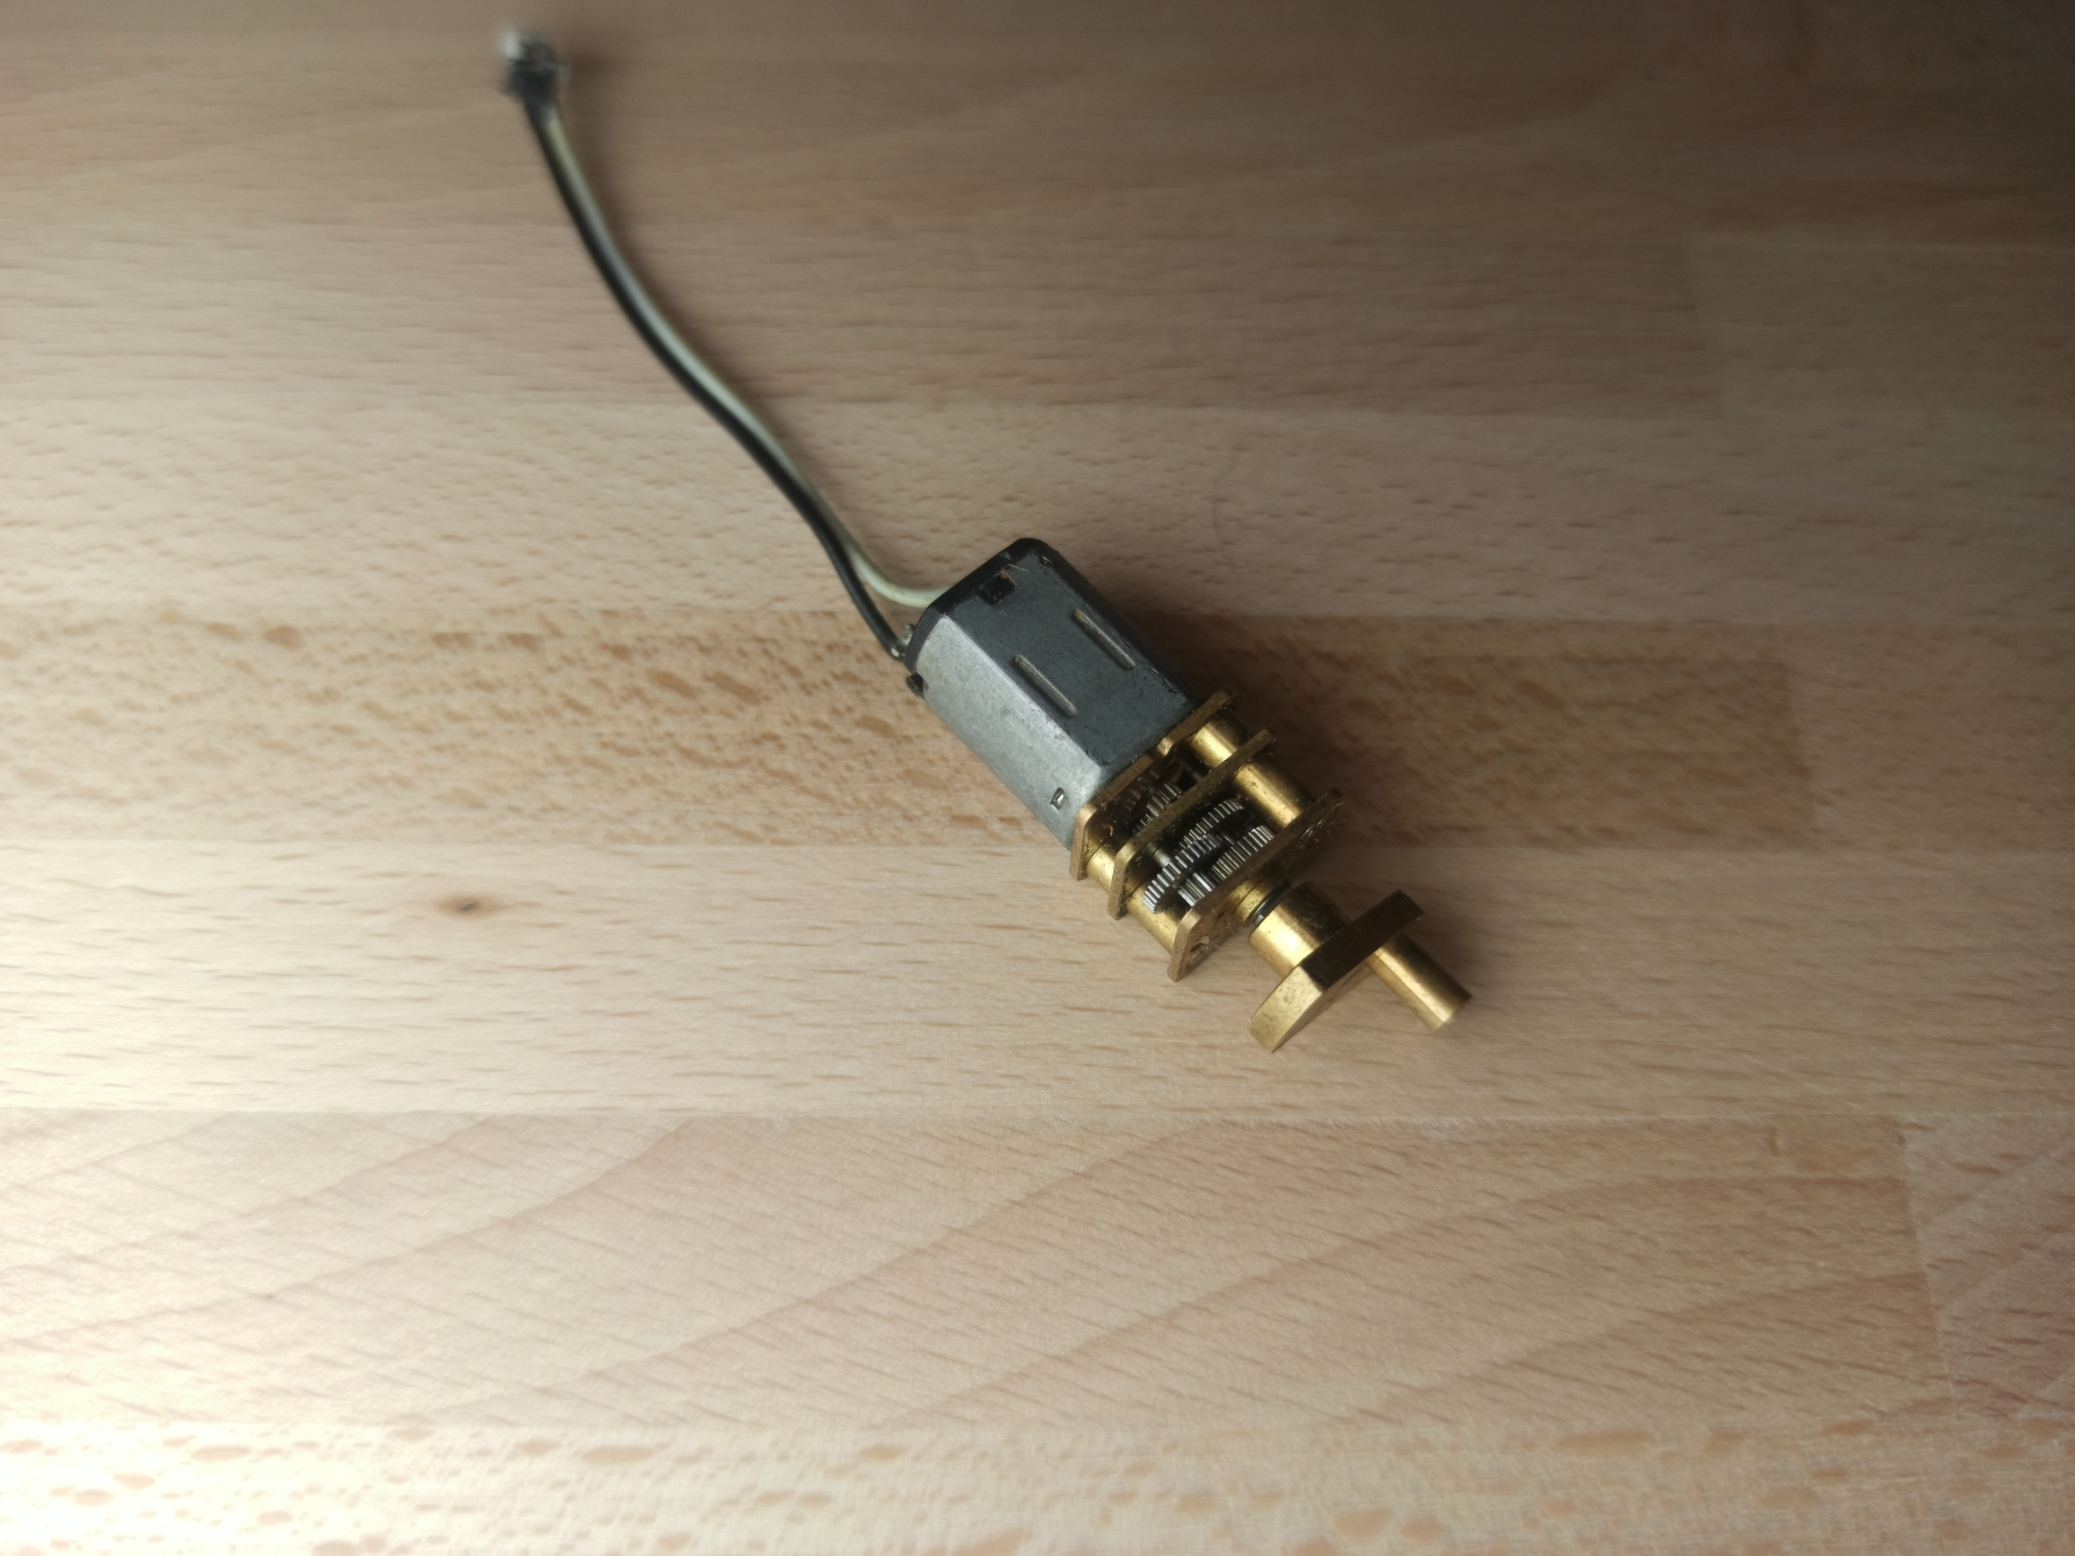
\includegraphics[width=160pt]{kapitoly/obrazky/E3/motory/hodinovyStrojek.jpg}
    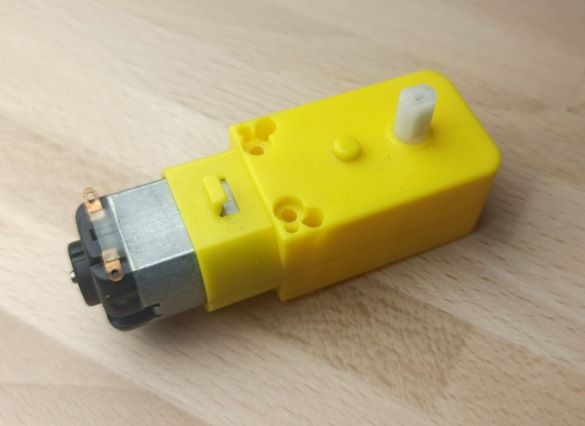
\includegraphics[width=160pt]{kapitoly/obrazky/E3/motory/zluty_motor.jpg}
    \caption{fotografie obou testovaných motorů} 
    \label{fig:E3-motory}
\end{figure}

\begin{figure}[htbp]
    \centering
    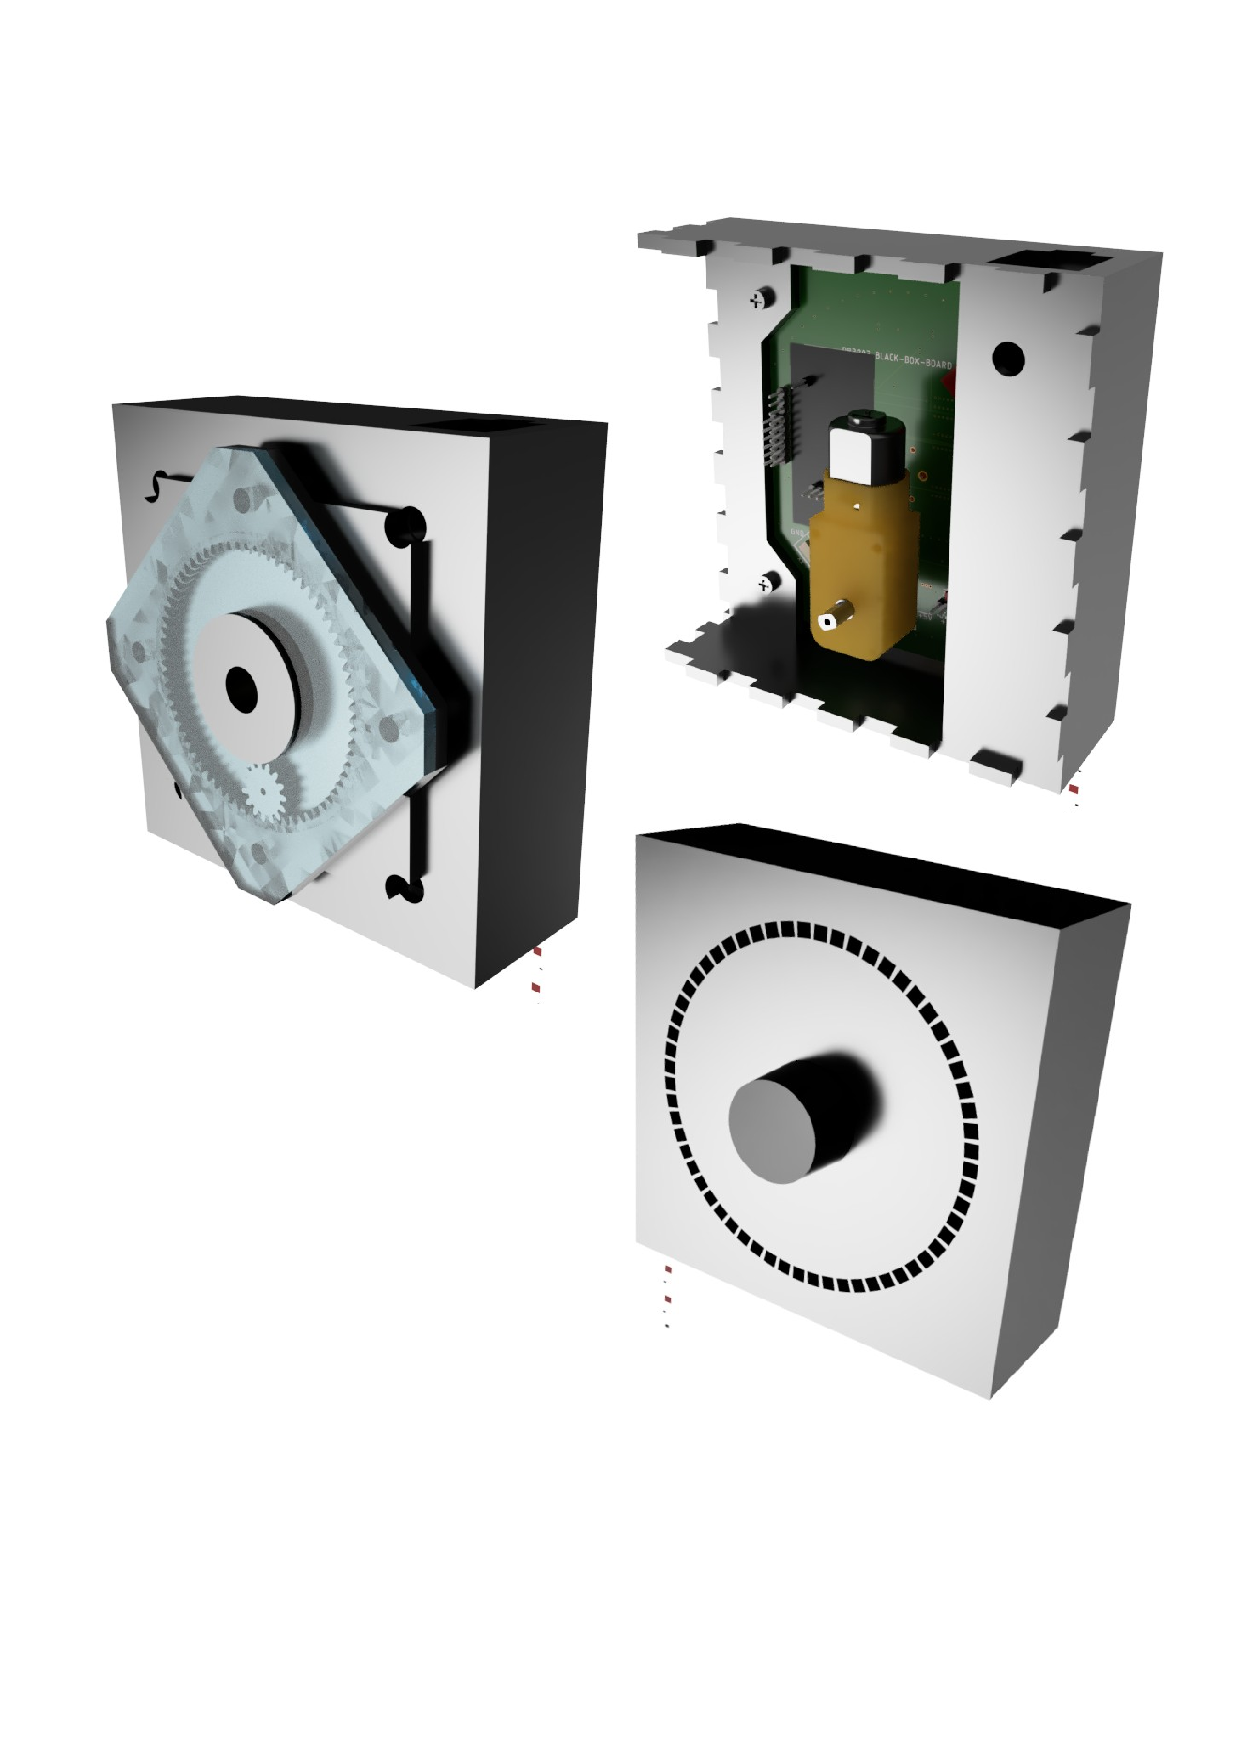
\includegraphics[width=\textwidth]{kapitoly/obrazky/E3/rendery.pdf}
    \caption{render varianty E3}
    \label{fig:E3-renderi}
\end{figure}

Přes velké množství funkcí jsem ale opět koncept přepracoval. Hlavním důvodem změn bylo náročné uložení rotační západky, 
které vyžadovalo ozubený věnec a několik dalších tisknutých dílů.

\newpage